
\begin{flushleft}
	\begin{itemize}
		\item A unit is a systemd object that performs or controls a particular task or action. 
		\item Systemd uses units to:
		\begin{itemize}
			\item start/stop/manage services
			\item organize boot process
			\item maintain tasks and processes
			\item create sockets
			\item mount file-system
			\item initialize hardware
		\end{itemize}
		\item A systemd unit consists of a name, type, and configuration file.
		\item Command to list available unit types:
		\begin{tcolorbox}[breakable,notitle,boxrule=1pt,colback=black,colframe=black]
			\color{green}
			\fontdimen2\font=1em
			\# systemctl -t help
			\fontdimen2\font=4pt
		\end{tcolorbox}
		
		\begin{figure}[h!]
			\centering
			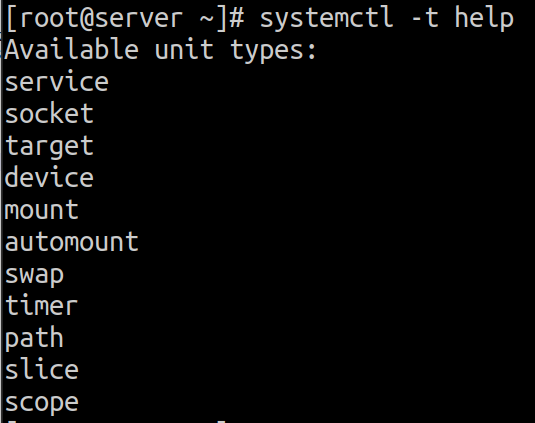
\includegraphics[scale=.5]{content/chapter1/images/units.png}
			\caption{Sample output}
			\label{fig:mascot}
		\end{figure}	
	
		\item Command to list all units of a specific type:		
		\begin{tcolorbox}[breakable,notitle,boxrule=1pt,colback=black,colframe=black]
			\color{green}
			\fontdimen2\font=1em
			\# systemctl ---type=service
			\newline
			\# systemctl ---type=socket
			\newline
			\# systemctl ---type=mount
			\fontdimen2\font=4pt
		\end{tcolorbox}
		
	\end{itemize}
		

	\newpage
	

	\textbf{Location of systemd units file:}
	\begin{itemize}
		\item \textbf{/usr/lib/systemd/system/}
		\item \textbf{/etc/systemd/system/}
	\end{itemize}
	
	\textbf{Some common unit types are listed as follows:}
	\begin{itemize}
		\item \textbf{Service units}:
		\begin{itemize}
			\item Service units represent system services.
			\item They have a \textbf{".service"} extension.
			\item Used to start/stop/restart/reload daemons, such as a web server.
			\item Eg: sshd.service unit file is at /usr/lib/systemd/system/sshd.service
		\end{itemize}
		\bigskip\bigskip
		\item \textbf{Socket units}:
		\begin{itemize}
			\item What is a socket? A socket consists of the IP address of a system and the port number of a program within the system. 
			\begin{figure}[h!]
				\centering
				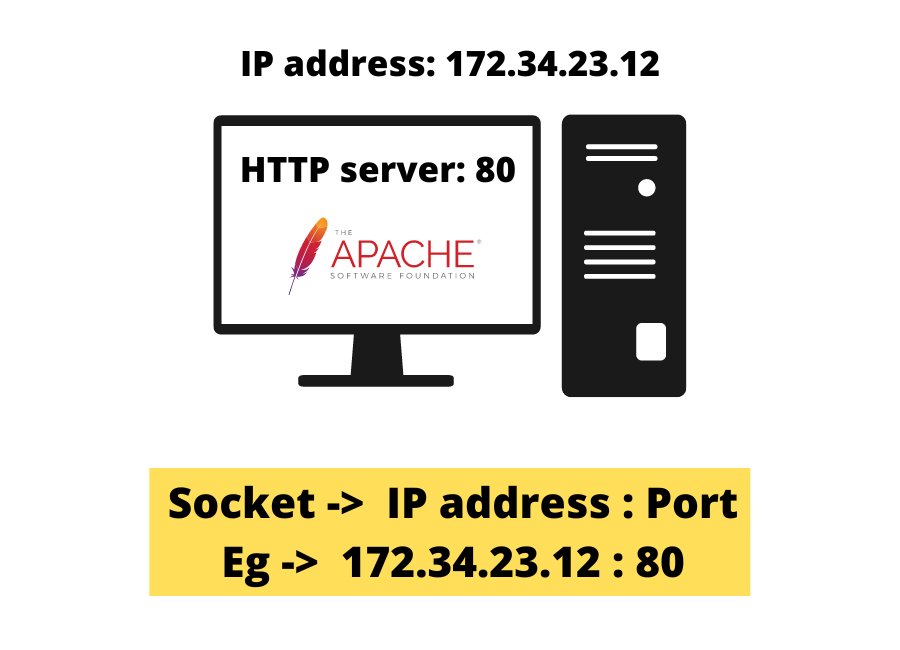
\includegraphics[scale=0.4]{content/chapter1/images/socket.png}
				\caption{Socket}
				\label{fig:socket1}
			\end{figure}
			\item A socket unit listen on an IP address and a port, and when something connects to it, the socket is handed over to the daemon it is made for.
			\item They have a \textbf{".socket"} extension.
			\item They represent interprocess communication (IPC) sockets.	
			\item Eg: dbus.socket unit file is at /usr/lib/systemd/system/dbus.socket
		\end{itemize}
		\bigskip \bigskip
		\item \textbf{Target units}:
		\begin{itemize}
			\item Targets are used for grouping and ordering units. 
			\item At different targets, different services, sockets, and other units are started.
			\item They have a \textbf{".target"} extension.
			\item Eg: multi-user.target unit file is at /usr/lib/systemd/system/multi-user.target
		\end{itemize}
		

	\end{itemize}
	
\end{flushleft}

\newpage

